\section{Evaluation}
\label{sec:evaluation}

To keep the main-body evaluation focused,
we report the load-bearing live experiments for each research question --
the malicious-proposer attack and the P2P quorum-gate result for RQ1, the
composite-fault stress test and the seven-scenario fault-injection sweep
for RQ2, the hysteresis parameter sweep for RQ3, and the extended-proposal
overhead benchmark for RQ4 -- out of a ten-experiment suite. The remaining
attack scenarios and a secondary ZK-backend comparison are reported in
Appendix~\ref{app:attacks} and Appendix~\ref{app:backend}; a Bitcoin-reorg
boundary test is reported in Appendix~\ref{app:reorg}. Unless noted
otherwise, every number below is a live measurement on the real 7-validator
testbed (Section~\ref{sec:setup}), not an in-process simulation; the
malicious-proposer test below is the one exception, run at 4-node scale as
disclosed in Section~\ref{sec:setup}.

\label{subsec:rq1}

\textbf{Malicious proposer.} We selected the malicious-proposer scenario as
our first representative attack because it directly exercises the extended
proposal's core safety property: a Byzantine leader that fabricates its
FSM-state claim. In this scenario, a compromised validator (25\% of voting
power at 4-node scale) is configured to broadcast a proposal whose FSM-state
field does not match its own honest sensor readings. Across
the live run, \textbf{safety held with zero AppHash divergence}: every
honest validator's independent re-evaluation of the FSM's own transition
function rejected the forged claim at the
proposal-validation step, consistent with the \emph{Strict FSM Transition
Safety} and \emph{Accountability} properties verified in
Section~\ref{sec:formal}. This result is one row of a broader ten-scenario
attack suite covering eclipse, Sybil, data withholding, forged Bitcoin
receipts, withdrawal-during-\textsc{Sovereign}, censorship, a combined
attack, double-signing, and timeout flooding, all of which held safety with
zero divergence; the full per-attack results are reported in
Appendix~\ref{app:attacks}.

\textbf{P2P quorum gate.} Our second RQ1 result addresses a different
safety property: does the tri-interface P2P profiler (Section~\ref{subsec:sensors})
translate into a real consensus safeguard, or only a monitoring signal? We
compare it against a peer-count-only baseline across four synthetic attacks
via a 2{,}000-trial-per-cell Monte Carlo study, then confirm the two most
diagnostic attacks live on the real cluster.

\begin{table}[h]
\caption{P2P Detector Accuracy: Tri-Interface vs.\ Peer-Count-Only (Synthetic, 2{,}000 trials/cell)}
\label{tab:p2p-detector}
\centering
\footnotesize
\begin{tabular}{@{}lrr@{}}
\toprule
\textbf{Attack} & \textbf{Detection delay (snapshots)} & \textbf{Evasion threshold} \\
\midrule
P1 Peer-slot exhaustion & 2.23 & 0.17 \\
P2 Multi-subnet Sybil & 1.00 & 0.00 \\
P3 Churn-based rotation & 1.70 & 0.12 \\
P4 Relay-node latency & 2.71 & 0.25 \\
\bottomrule
\end{tabular}
\\[2pt]
\footnotesize Peer-count-only baseline: 100\% false-negative rate and an
evasion threshold of 1.0 (never caught, at any intensity) on all four
attacks, by construction -- all four preserve clean-peer count. The
tri-interface profiler holds 0\% false positives and 0\% false negatives on
every attack.
\end{table}

Table~\ref{tab:p2p-detector} shows the tri-interface profiler catches every
attack a peer-count-only detector is structurally blind to, across the full
range of intensities an adaptive adversary could search (evasion threshold
$\leq 0.25$ in every case), and this advantage is stable across three
different attack-ramp shapes (linear, front-loaded, stealthy-slow; 300/300
trials caught in every shape$\times$attack cell) and independent of
concurrent Bitcoin/DA degradation. Live confirmation isolates a subtler
finding than raw detection accuracy: a real quorum gate on top of that
detection. Attack P3 (churn-based rotation, eight repeated container
restart cycles on 2 of 7 proposers, $\sim$29\% of voting power)
is correctly \emph{sensed} -- the peer-churn-rate metric on both attacked nodes
crosses the detection threshold -- yet produces \textbf{no committed FSM
transition}, because a transition requires $\geq 2f{+}1$ voting
power's signed observations before it commits, and a
minority-visible degradation cannot supply that quorum. Attack P4
(sustained 350$\pm$50\,ms delay on all of one validator's real P2P
interfaces, visible to 7 of 7 validators, i.e.\ full quorum) produces the
opposite outcome: a full, correctly-bounded
\textsc{Anchored}$\to$\textsc{Suspicious}$\to$\textsc{Sovereign} cascade
(+39\,s, +72\,s relative to the attack start) that holds for the entire
244-second attack window and recovers
(\textsc{Recovering}$\to$\textsc{Anchored}) within 5 seconds of the delay
clearing, as shown in Fig.~\ref{fig:a4-cascade}.

\begin{figure}[h]
\centering
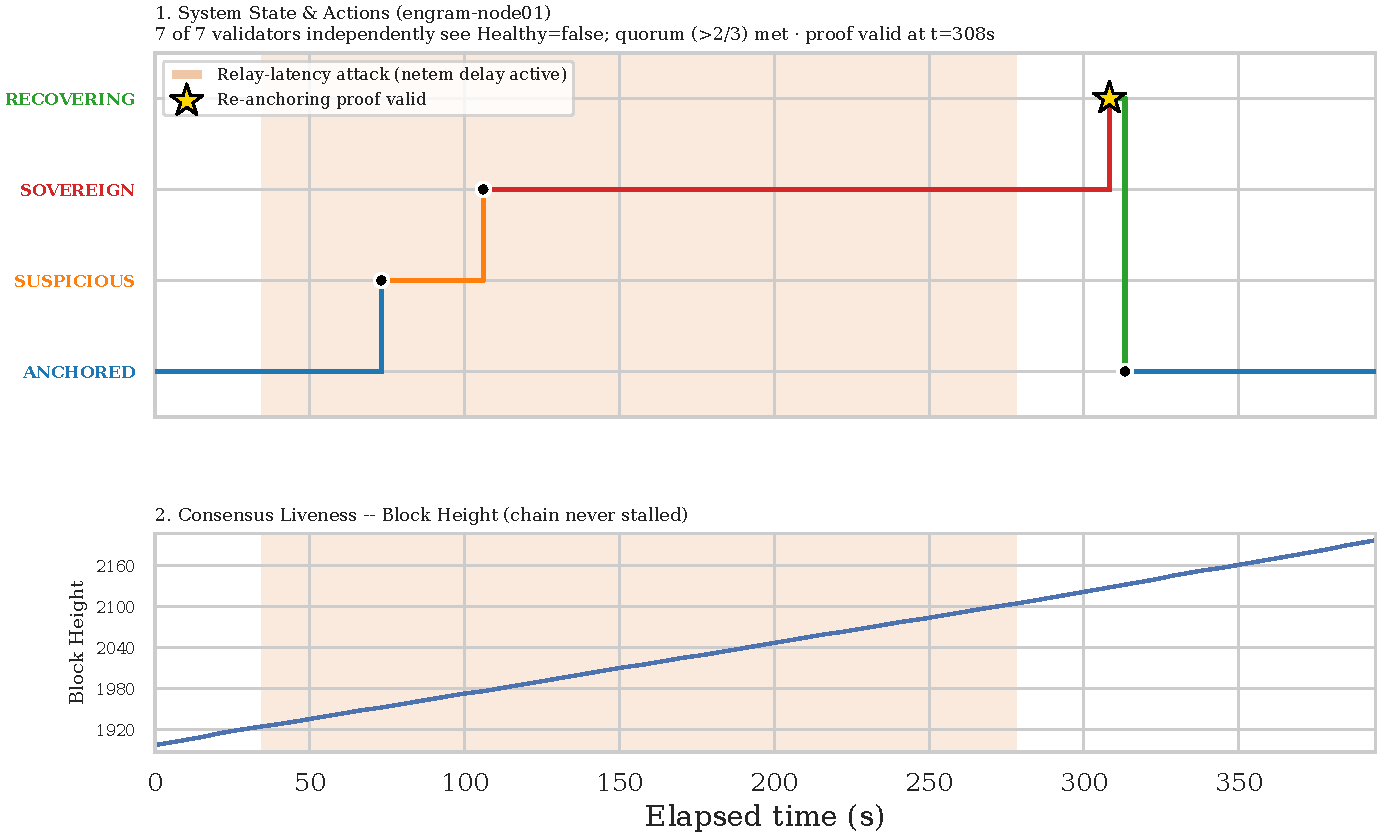
\includegraphics[trim=0 0 0 38pt, clip, width=\linewidth]{figures/figure5_a4_cascade_timeline_live.pdf}
\caption{FSM cascade under a real, quorum-visible P2P relay-latency attack
(P4): all 7 validators independently sense the degradation, the transition
commits once quorum is met, and block production (bottom panel) never
stalls through the cascade or the recovery.}
\label{fig:a4-cascade}
\end{figure}

Together, P3 and P4 are two outcomes of one mechanism, not two separate
detector results: the identical class of real, sensor-confirmed P2P
degradation is correctly blocked from committing when only a minority of
validators observes it, and correctly drives a bounded, liveness-preserving
state cascade when a supermajority does. This is a specific instance of the
safety property RQ1 asks for -- resistance to a Byzantine-influenced
minority forcing an unwarranted state transition -- though we note it
exercises the quorum-threshold mechanism under adversarial network
conditions rather than the forged-receipt or data-withholding vectors RQ1
also names; those are addressed separately by the malicious-proposer result
above and by Appendix~\ref{app:attacks}'s broader attack suite.

\label{subsec:rq2}

\textbf{Composite fault.} To answer RQ2 we first ran a single, continuous,
scripted composite-fault sequence rather than isolated single-fault
scenarios: growing Bitcoin congestion, layered onto a full Celestia DA
outage (all seven independent bridges stopped together), layered onto three
cycles of packet loss on the validator P2P network, all three overlapping
at their peak, followed by a sequential, real recovery -- run under a
standing wide-area-network latency baseline. Fig.~\ref{fig:fsm-timeline}
plots the resulting FSM state timeline.

\begin{figure}[h]
\centering
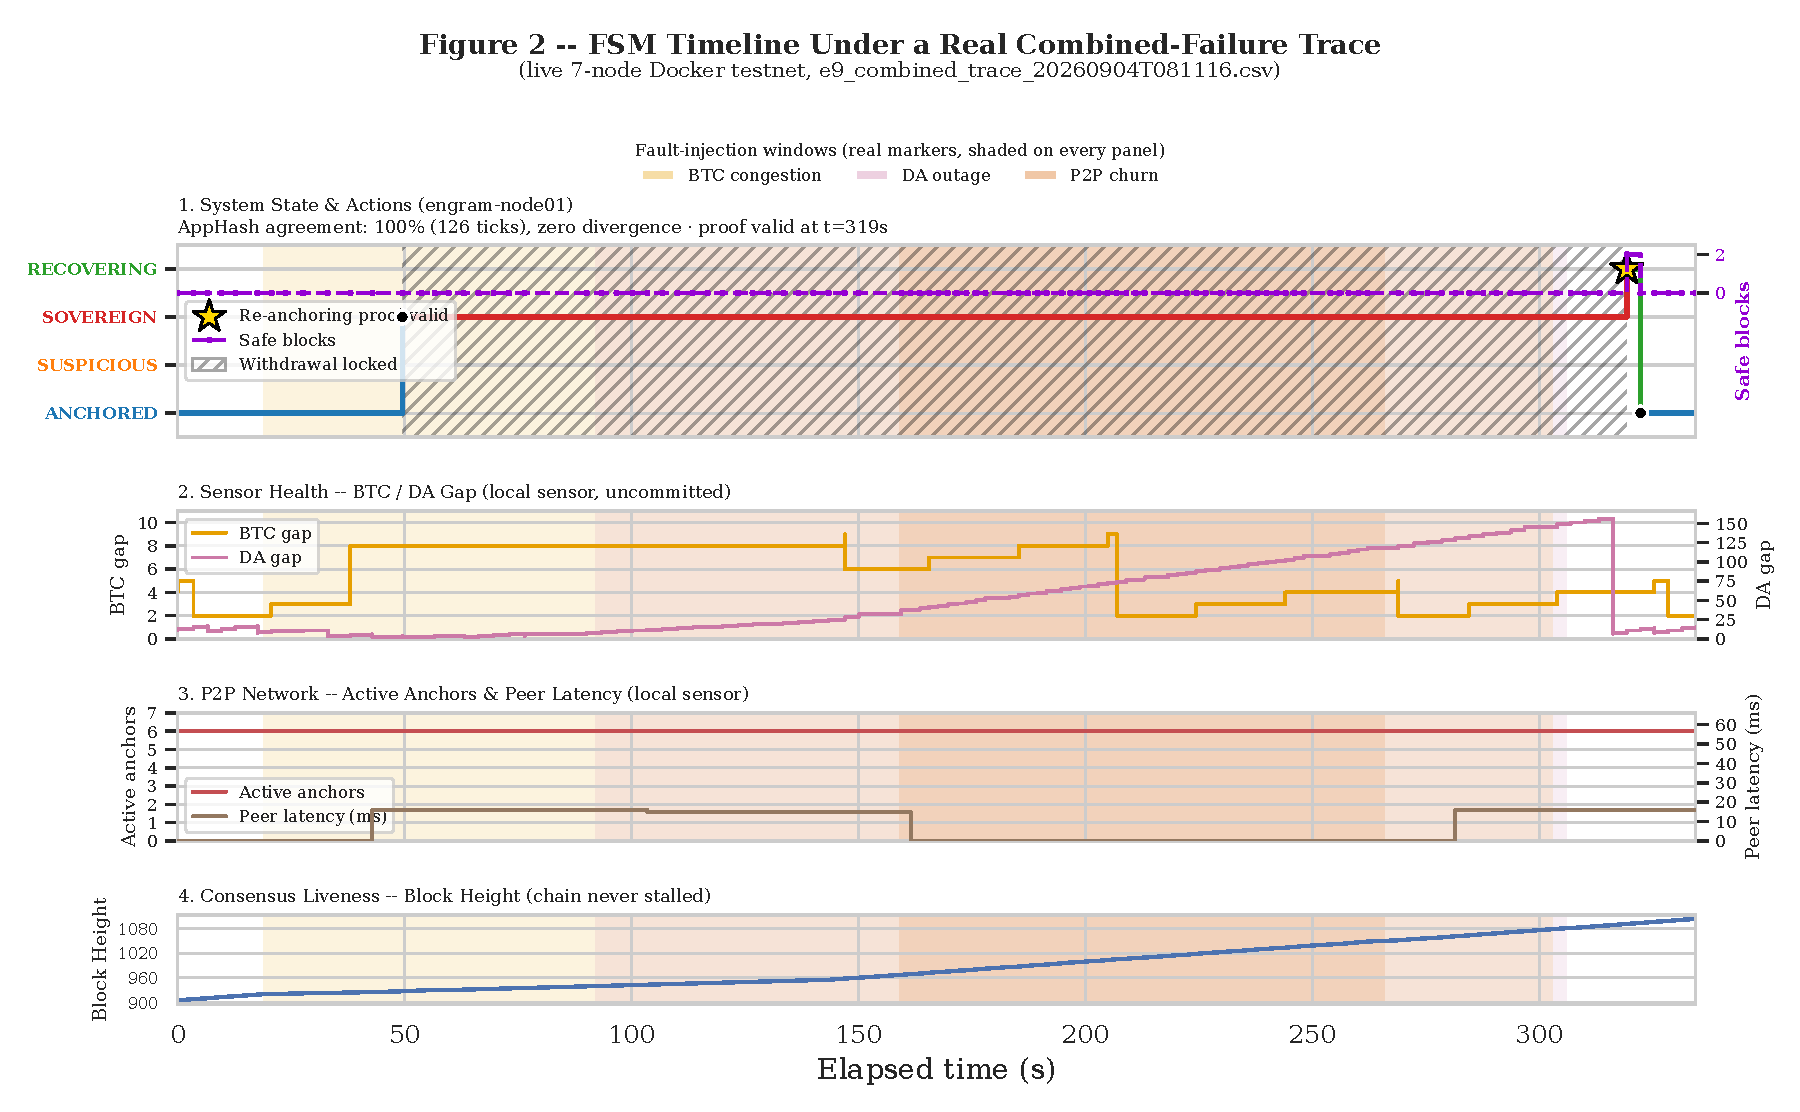
\includegraphics[trim=0 0 0 40pt, clip, width=0.95\linewidth]{figures/figure2_trace_timeline_live.pdf}
\caption{FSM state timeline, sensor readings, P2P network state, and block
height under a layered composite fault sequence (Bitcoin congestion + DA
outage + P2P churn, overlapping at their peak).}
\label{fig:fsm-timeline}
\end{figure}

Over a 341-second run (742 samples, 126 polling ticks), the chain height
progressed continuously from 905 to over 1093 with \textbf{no stalled
round}, and all seven validators reached \textbf{100\% AppHash agreement}
across every tick, with zero divergent heights and zero RPC errors. The
chain reached \textsc{Sovereign} under the combined fault, then completed a
real recovery cycle -- \textsc{Recovering} at $t{=}321$\,s,
\textsc{Anchored} at $t{=}324$\,s -- once the injected faults were healed.
Withdrawals were locked for the entire \textsc{Sovereign}/\textsc{Recovering}
window and unlocked only after the transition back to \textsc{Anchored},
matching the circuit-breaker invariant of Section~\ref{sec:formal}; the
re-anchoring proof (Section~\ref{subsec:reanchoring}) was confirmed valid at
$t{=}319$\,s, ahead of the state transition it gates.

\textbf{Seven-scenario fault-injection sweep.} The composite trace shows
the mechanism survives worst-case overlap, but does not isolate which
failure mode drives which behavior. We complement it with a longer,
864-second live run walking the chain through seven sequential scenarios --
S1 normal baseline, S2 Bitcoin congestion, S3 DA outage, S4 partial P2P
eclipse, S5 total anchor isolation, S6 combined Bitcoin+DA failure, and S7
recovery -- each building on the last, with 153 real FSM transitions logged
across all 7 validators. Fig.~\ref{fig:s1-s7} plots the full continuous
timeline.

\begin{figure}[h]
\centering
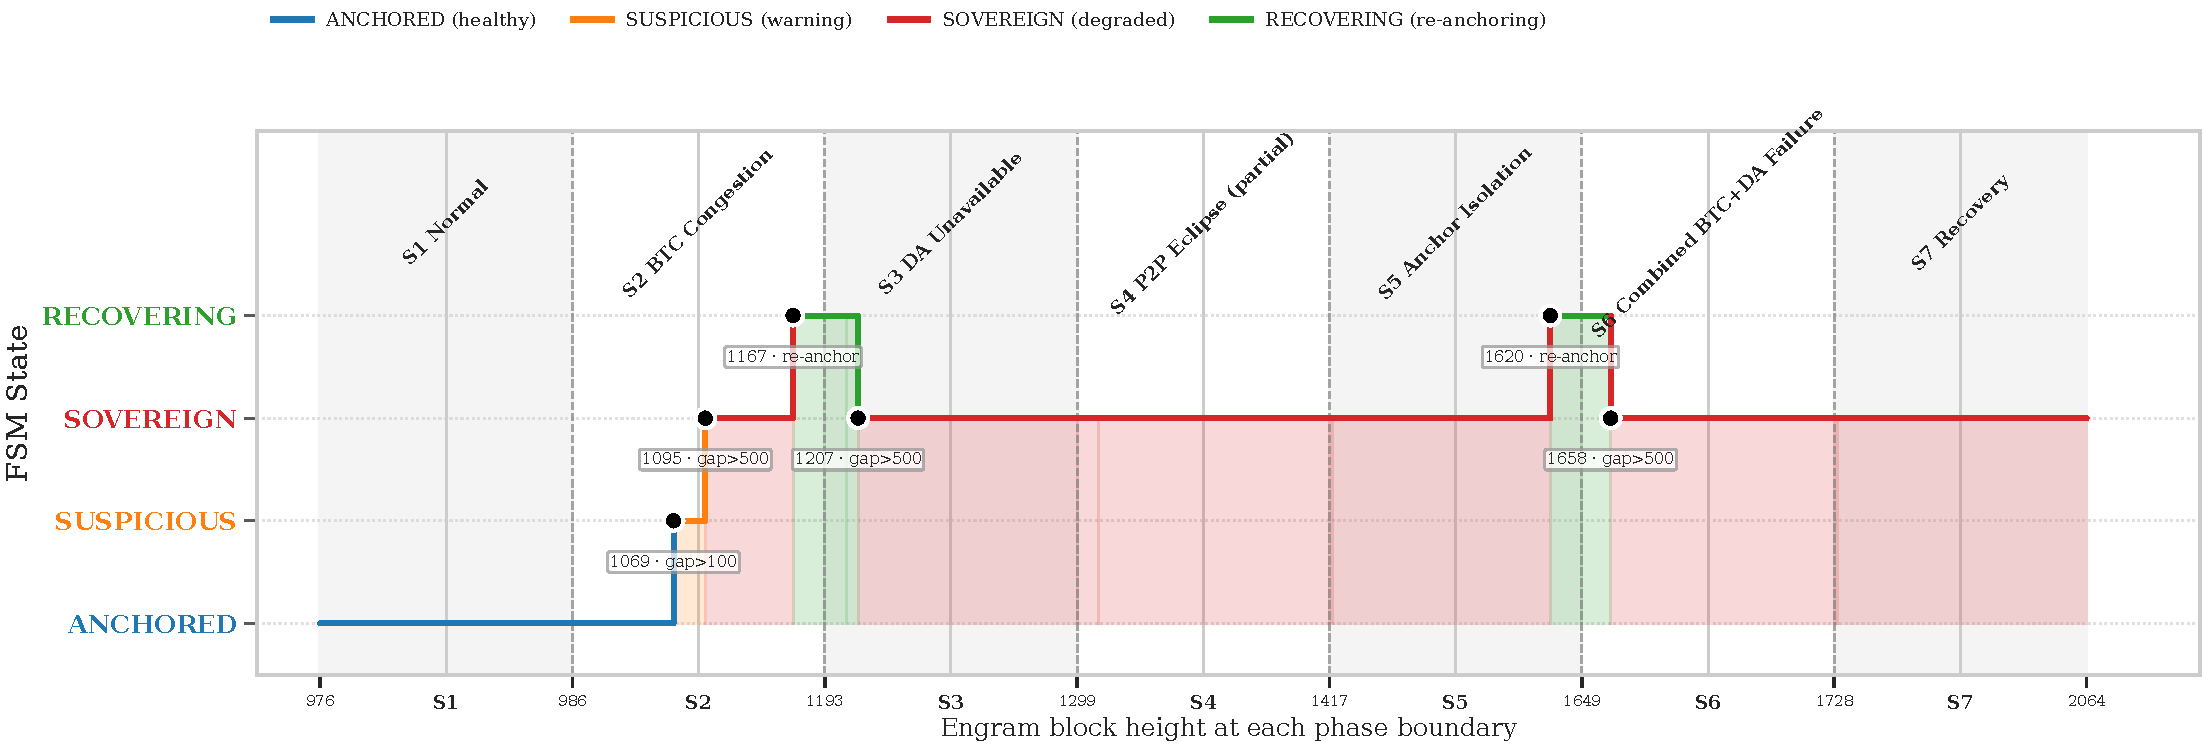
\includegraphics[trim=0 0 0 22pt, clip, width=0.95\linewidth]{figures/figure3_single_timeline_live.pdf}
\caption{Continuous FSM-state timeline across seven sequential
fault-injection scenarios (S1--S7), true block-height ranges, live
7-validator testbed. Each scenario begins where the previous scenario's
recovery ended.}
\label{fig:s1-s7}
\end{figure}

Every scenario shows the correct qualitative response: S2 (Bitcoin
congestion) and S3 (DA outage) each independently escalate through
\textsc{Suspicious} to \textsc{Sovereign} and recover; S4 (partial P2P
eclipse) escalates fully to \textsc{Sovereign}, while S5 (total anchor
isolation on one of seven validators) only ever produces a transient,
hysteresis-absorbed \textsc{Suspicious} dip that self-heals, because losing
1 of 7 anchor peers does not zero out the active-anchor-peer count and therefore
never satisfies the immediate-escalation condition -- a direct, live
confirmation that S4 and S5 are qualitatively different failure classes, not
two instances of the same detector saturating; S6 (Bitcoin and DA failing
together) escalates directly to \textsc{Sovereign}; and S7 (recovery) closes
the loop back to \textsc{Anchored} via a real submitted re-anchoring proof.
Two results from this run are worth highlighting beyond the qualitative
pattern. First, S2 itself shows two brief, real \textsc{Suspicious} blips
(19--22\,s and 77--80\,s into the scenario) that hysteresis absorbs back to
\textsc{Anchored} before the scenario's real escalation at 141\,s -- the
first confirmation on physical infrastructure that hysteresis absorbs
genuine noise, a
property previously shown only in E5's synthetic sweeps
(Section~\ref{subsec:rq3}). Second, per-scenario throughput held
close to baseline throughout: block-interval means ranged 1.30--1.93\,s
across all seven scenarios (vs.\ 1.34\,s at the S1 healthy baseline), with
the two heaviest scenarios (S4 partial eclipse and S7 recovery) showing the
largest, but still bounded, tail latency (p95 4.27\,s and 3.10\,s
respectively). Together with the composite-fault result above, this
answers RQ2 affirmatively from two complementary angles: the chain keeps
committing blocks under both an overlapping worst-case fault and under each
individual failure mode in isolation, and recovers correctly in every case,
rather than halting.

\label{subsec:rq3}

RQ3 asks whether hysteresis prevents oscillation (``flapping'') once
peripherals recover, without unduly delaying recovery. We swept the
governing threshold on each of the three hysteresis-gated edges --
\textsc{Recovering}$\to$\textsc{Anchored},
\textsc{Anchored}$\to$\textsc{Suspicious}, and
\textsc{Suspicious}$\to$\textsc{Anchored} -- both in-process (fixed-seed
synthetic noise, for a clean monotonic baseline) and live on the real
7-validator cluster (real network noise, which does not cancel out the way
a fixed seed does). Fig.~\ref{fig:hysteresis} plots the resulting
uptime/absorption trade-off for all three edges.

\begin{figure}[h]
\centering
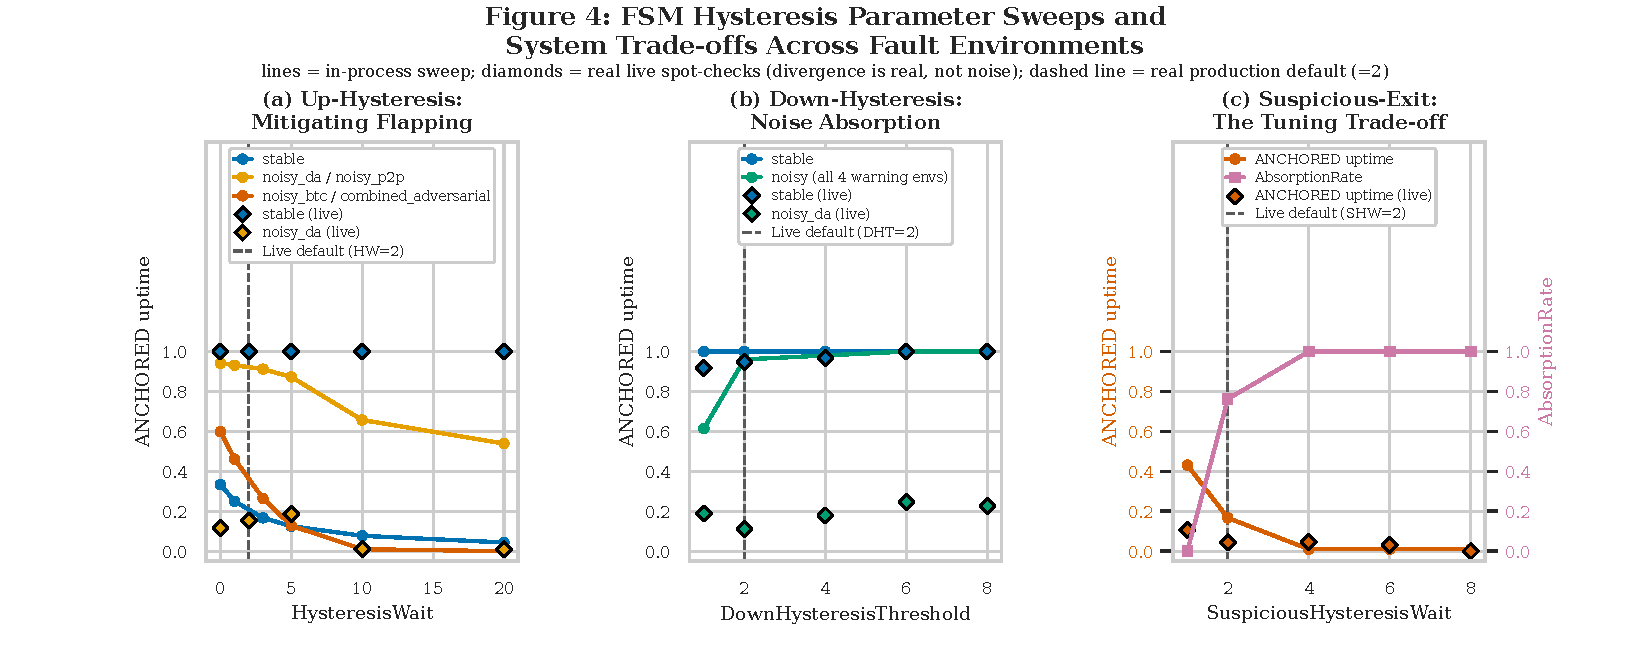
\includegraphics[trim=0 0 0 28pt, clip, width=0.95\linewidth]{figures/figure4_hysteresis_tradeoffs.pdf}
\caption{Hysteresis parameter sweep across all three absorb edges. Lines:
in-process sweep under different noise profiles; diamonds: live spot-checks
on the real 7-validator cluster (divergence from the in-process line is
real network behavior, not measurement noise); dashed line: the protocol's
live production default.}
\label{fig:hysteresis}
\end{figure}

\begin{table}[h]
\caption{Down-Hysteresis Sweep (\textsc{Anchored}$\to$\textsc{Suspicious}),
In-Process}
\label{tab:hysteresis-down}
\centering
\footnotesize
\begin{tabular}{@{}lrrrrr@{}}
\toprule
\textbf{Threshold} & 1 & 2 & 4 & 6 & 8 \\
\midrule
Flapping (count)     & 31 & 1 & 1 & 0 & 0 \\
Anchored uptime (\%) & 61.39 & 96.04 & 98.02 & 100.00 & 100.00 \\
Absorption rate (\%) & 0.00 & 94.74 & 95.24 & 100.00 & 100.00 \\
\bottomrule
\end{tabular}
\end{table}

Table~\ref{tab:hysteresis-down} shows the clearest single result: on the
\textsc{Anchored}$\to$\textsc{Suspicious} edge, raising the down-hysteresis
threshold from 1 to 4 collapses flapping from 31 events to 1 and raises
anchored uptime from 61.4\% to 98.0\%, and the absorption rate saturates
near 100\% by threshold 4--6. The live spot-check on the real cluster
confirms this is not merely a synthetic artifact but shows a stronger,
practically important finding: under real wide-area-network jitter alone
(with \emph{no} injected fault), thresholds 1, 2, and even 4 still produced
spurious flapping, and only threshold $\geq 6$ was clean (0 flapping, 100\%
uptime) -- a materially stronger requirement than the protocol's own default
value of 2, and a concrete, actionable recommendation for deployment in a
WAN-realism regime. We flag an apparent tension we have not resolved: the
composite-fault, seven-scenario, and P4 experiments above all ran at this
same default threshold of 2 under the same WAN-jitter baseline, yet report
no comparable flapping. This is not necessarily a contradiction --
this dedicated sweep is the only experiment that explicitly counts
flapping events in isolation from any other injected fault; the other
experiments track qualitative correctness (AppHash agreement, block
production) rather than a flapping count, so an occasional spurious flap
not large enough to affect those outcomes would not have been visible in
their results either way. We report this as a difference in measurement
scope, not as evidence that the other experiments were in fact flap-free.
The symmetric edges show consistent trade-offs in the
opposite direction: on the \textsc{Recovering}$\to$\textsc{Anchored} edge, a
larger hysteresis-wait threshold strictly reduces anchored uptime under
sustained critical-level noise (59.8\%$\to$0.0\% as the threshold goes from
0 to 20) -- a designed, expected negative result, since critical-level
conditions bypass hysteresis by construction rather than being absorbed by
it. On the \textsc{Suspicious}$\to$\textsc{Anchored} edge, absorption rate
rises from 0\% to 100\% as the threshold goes from 1 to 4, but this is a
genuine trade-off, not a free improvement: the same accumulating
suspicious-state duration timer that a longer threshold is meant to
outlast can independently force escalation to \textsc{Sovereign} once it
hits its own cap, so only the smallest threshold values in our sweep
(1--2) actually reached \textsc{Anchored} within the timeout window. We
discuss the resulting open design question -- asymmetric hardening across
edges -- in Section~\ref{sec:discussion}. Appendix~\ref{app:reorg} reports a
complementary recovery-boundary result: how far a real Bitcoin
reorganization can go before the same FSM reacts at all.

\label{subsec:rq4}

\begin{table}[h]
\caption{Extended Proposal Overhead vs.\ Vanilla CometBFT}
\label{tab:overhead}
\centering
\footnotesize
\begin{tabular}{@{}lrr@{}}
\toprule
\textbf{Metric} & \textbf{Vanilla} & \textbf{Engram (extended)} \\
\midrule
Steady-state proposal tax & 0 B/block & +228 B/block \\
Full proposal-validation CPU & --- & 18{,}252 ns \\
p95 commit latency @ 20 tx/s & 1.017 s & 1.021 s \\
Blocks/s @ 20 tx/s ($n{=}5$) & 0.953 $\pm$ 0.007 & 0.743 $\pm$ 0.008 \\
Tx-accepted/s @ 20 tx/s & 20.00 $\pm$ 0.00 & 19.99 $\pm$ 0.00 \\
\bottomrule
\end{tabular}
\end{table}

Table~\ref{tab:overhead} answers RQ4 directly. On the healthy path, the
extended proposal adds a small, near-constant \textbf{+228 bytes per block}
(100\% of blocks carry the marker) versus zero for vanilla CometBFT; a live
376-block sample confirms 100\% marker coverage with per-state average
proposal sizes of 247--270 bytes, and the one recovery-proof-carrying block
observed matched the expected $\sim$14.7\,KB proof-plus-envelope size from
Section~\ref{subsec:reanchoring}. Validation CPU cost is negligible: the
full proposal-validation path costs 18{,}252\,ns (18.25\,$\mu$s) on a
steady-state, non-recovery block -- several orders of magnitude below both
CometBFT's own commit-timeout parameter (hundreds of milliseconds) and this
cluster's $\sim$1-second block interval. Under load ramped from 5 to 100
tx/s, we found \textbf{no throughput ceiling within the tested range}:
every rate stage accepted
100\% of submitted transactions in both modes, and p95 commit latency
stayed essentially flat ($\sim$1.01--1.02\,s) regardless of rate, dominated
by the block interval rather than load. At a fixed rate of 20 tx/s with
$n{=}5$ independent repeats, the extended mode's block-production rate
(0.743 $\pm$ 0.008 blocks/s) was consistently, but modestly, lower than
vanilla's (0.953 $\pm$ 0.007 blocks/s) -- a stable $\sim$23--27\% gap in
per-round overhead (Cohen's $d{=}$--25.3, a very large but tightly
reproducible effect) that a throughput-corrected metric shows converges
between the two modes, indicating the gap is round-skip overhead rather than
a growing backlog. We regard this as an acceptable, bounded cost given the
liveness and safety guarantees demonstrated under RQ1--RQ3.